\documentclass{ximera}
\graphicspath{  %% When looking for images,
{./}            %% look here first,
{./pictures/}   %% then look for a pictures folder,
{../pictures/}  %% which may be a directory up.
{../../pictures/}  %% which may be a directory up.
{../../../pictures/}  %% which may be a directory up.
{../../../../pictures/}  %% which may be a directory up.
}

\usepackage{listings}
%\usepackage{circuitikz}
\usepackage{xcolor}
\usepackage{amsmath,amsthm}
\usepackage{subcaption}
\usepackage{graphicx}
\usepackage{tikz}
%\usepackage{tikz-3dplot}
\usepackage{amsfonts}
%\usepackage{mdframed} % For framing content
%\usepackage{tikz-cd}

  \renewcommand{\vector}[1]{\left\langle #1\right\rangle}
  \newcommand{\arrowvec}[1]{{\overset{\rightharpoonup}{#1}}}
  \newcommand{\ro}{\texttt{R}}%% row operation
  \newcommand{\dotp}{\bullet}%% dot product
  \renewcommand{\l}{\ell}
  \let\defaultAnswerFormat\answerFormatBoxed
  \usetikzlibrary{calc,bending}
  \tikzset{>=stealth}
  




%make a maroon color
\definecolor{maroon}{RGB}{128,0,0}
%make a dark blue color
\definecolor{darkblue}{RGB}{0,0,139}
%define the color fourier0 to be the maroon color
\definecolor{fourier0}{RGB}{128,0,0}
%define the color fourier1 to be the dark blue color
\definecolor{fourier1}{RGB}{0,0,139}
%define the color fourier 1t to be the light blue color
\definecolor{fourier1t}{RGB}{173,216,230}
%define the color fourier2 to be the dark green color
\definecolor{fourier2}{RGB}{0,100,0}
%define teh color fourier2t to be the light green color
\definecolor{fourier2t}{RGB}{144,238,144}
%define the color fourier3 to be the dark purple color
\definecolor{fourier3}{RGB}{128,0,128}
%define the color fourier3t to be the light purple color
\definecolor{fourier3t}{RGB}{221,160,221}
%define the color fourier0t to be the red color
\definecolor{fourier0t}{RGB}{255,0,0}
%define the color fourier4 to be the orange color
\definecolor{fourier4}{RGB}{255,165,0}
%define the color fourier4t to be the darker orange color
\definecolor{fourier4t}{RGB}{255,215,0}
%define the color fourier5 to be the yellow color
\definecolor{fourier5}{RGB}{255,255,0}
%define the color fourier5t to be the darker yellow color
\definecolor{fourier5t}{RGB}{255,255,100}
%define the color fourier6 to be the green color
\definecolor{fourier6}{RGB}{0,128,0}
%define the color fourier6t to be the darker green color
\definecolor{fourier6t}{RGB}{0,255,0}

%New commands for this doc for errors in copying
\newcommand{\eigenvar}{\lambda}
%\newcommand{\vect}[1]{\mathbf{#1}}
\renewcommand{\th}{^{\text{th}}}
\newcommand{\st}{^{\text{st}}}
\newcommand{\nd}{^{\text{nd}}}
\newcommand{\rd}{^{\text{rd}}}
\newcommand{\paren}[1]{\left(#1\right)}
\newcommand{\abs}[1]{\left|#1\right|}
\newcommand{\R}{\mathbb{R}}
\newcommand{\C}{\mathbb{C}}
\newcommand{\Hilb}{\mathbb{H}}
\newcommand{\qq}[1]{\text{#1}}
\newcommand{\Z}{\mathbb{Z}}
\newcommand{\N}{\mathbb{N}}
\newcommand{\q}[1]{\text{``#1''}}
%\newcommand{\mat}[1]{\begin{bmatrix}#1\end{bmatrix}}
\newcommand{\rref}{\text{reduced row echelon form}}
\newcommand{\ef}{\text{echelon form}}
\newcommand{\ohm}{\Omega}
\newcommand{\volt}{\text{V}}
\newcommand{\amp}{\text{A}}
\newcommand{\Seq}{\textbf{Seq}}
\newcommand{\Poly}{\textbf{P}}
\renewcommand{\quad}{\text{    }}
\newcommand{\roweq}{\simeq}
\newcommand{\rowop}{\simeq}
\newcommand{\rowswap}{\leftrightarrow}
\newcommand{\Mat}{\textbf{M}}
\newcommand{\Func}{\textbf{Func}}
\newcommand{\Hw}{\textbf{Hamming weight}}
\newcommand{\Hd}{\textbf{Hamming distance}}
\newcommand{\rank}{\text{rank}}
\newcommand{\longvect}[1]{\overrightarrow{#1}}
% Define the circled command
\newcommand{\circled}[1]{%
  \tikz[baseline=(char.base)]{
    \node[shape=circle,draw,inner sep=2pt,red,fill=red!20,text=black] (char) {#1};}%
}

% Define custom command \strikeh that just puts red text on the 2nd argument
\newcommand{\strikeh}[2]{\textcolor{red}{#2}}

% Define custom command \strikev that just puts red text on the 2nd argument
\newcommand{\strikev}[2]{\textcolor{red}{#2}}

%more new commands for this doc for errors in copying
\newcommand{\SI}{\text{SI}}
\newcommand{\kg}{\text{kg}}
\newcommand{\m}{\text{m}}
\newcommand{\s}{\text{s}}
\newcommand{\norm}[1]{\left\|#1\right\|}
\newcommand{\col}{\text{col}}
\newcommand{\sspan}{\text{span}}
\newcommand{\proj}{\text{proj}}
\newcommand{\set}[1]{\left\{#1\right\}}
\newcommand{\degC}{^\circ\text{C}}
\newcommand{\centroid}[1]{\overline{#1}}
\newcommand{\dotprod}{\boldsymbol{\cdot}}
%\newcommand{\coord}[1]{\begin{bmatrix}#1\end{bmatrix}}
\newcommand{\iprod}[1]{\langle #1 \rangle}
\newcommand{\adjoint}{^{*}}
\newcommand{\conjugate}[1]{\overline{#1}}
\newcommand{\eigenvarA}{\lambda}
\newcommand{\eigenvarB}{\mu}
\newcommand{\orth}{\perp}
\newcommand{\bigbracket}[1]{\left[#1\right]}
\newcommand{\textiff}{\text{ if and only if }}
\newcommand{\adj}{\text{adj}}
\newcommand{\ijth}{\emph{ij}^\text{th}}
\newcommand{\minor}[2]{M_{#2}}
\newcommand{\cofactor}{\text{C}}
\newcommand{\shift}{\textbf{shift}}
\newcommand{\startmat}[1]{
  \left[\begin{array}{#1}
}
\newcommand{\stopmat}{\end{array}\right]}
%a command to give a name to explorations and hints and theorems
\newcommand{\name}[1]{\begin{centering}\textbf{#1}\end{centering}}
\newcommand{\vect}[1]{\vec{#1}}
\newcommand{\dfn}[1]{\textbf{#1}}
\newcommand{\transpose}{\mathsf{T}}
\newcommand{\mtlb}[2][black]{\texttt{\textcolor{#1}{#2}}}
\newcommand{\RR}{\mathbb{R}} % Real numbers
\newcommand{\id}{\text{id}}
\newcommand{\coord}[1]{\langle#1\rangle}
\newcommand{\RREF}{\text{RREF}}
\newcommand{\Null}{\text{Null}}
\newcommand{\Nullity}{\text{Nullity}}
\newcommand{\Rank}{\text{Rank}}
\newcommand{\Col}{\text{Col}}
\newcommand{\Ef}{\text{EF}}
\newcommand{\boxprod}[3]{\abs{(#1\times#2)\cdot#3}}

\author{Zack Reed}
%borrowed from selinger linear algebra
\title{Cross Product}
\begin{document}
\begin{abstract}

\end{abstract}
\maketitle

\section*{Cross Product and its Properties}

 Here, we introduce the cross product, which has many applications in physics and engineering.  It also has important geometric properties.
 
\subsection*{Motivating the Cross Product}

Let's return to the unfinished problem of the previous section:

\begin{example}\name{Normal and standard equations}\label{exa:normal-from-three-points}

    Find normal and standard equations for the plane through the points
    $P = (0,1,3)$, $Q=(2,-1,0)$, and $R=(1,2,2)$.
  \end{example}
  
  \begin{solution}
    The goal is to find the normal vector to the plane so that we can more explicitly define the plane. For any vector $\vec{v}$, there is a nice linear transformation defined only on $\RR^3$, called the cross product and denoted $\vec{v}\times$, which will for any vector $\vec{u}$ give a third vector $\vec{w}$ that is orthogonal to both $\vec{v}$ and $\vec{u}$.

    This vector $\vec{w}=\vec{v}\times\vec{u}$ is exactly what we need to describe any plane from two vectors.

    First, let's find the two direction vectors and point that define the plane. If we center at $P$, we can use  $\longvect{PQ}$ and $\longvect{PR}$ as the planar direction vectors. 

    From the last section, we determined that the direction vectors are $\longvect{PQ}=\startmat{r} 2 \\ -2 \\ -3 \stopmat$ and $\longvect{PR}=\startmat{r} 1 \\ 1 \\ -1 \stopmat$.
    
    START HERE
    
    
    We can
    therefore use the cross product to compute a normal vector for the
    plane:
    \begin{equation*}
      \vect{n}
      ~=~
      \longvect{PQ} \times \longvect{PR}
      ~=~
      \startmat{r} 2 \\ -2 \\ -3 \stopmat
      \times
      \startmat{r} 1 \\ 1 \\ -1 \stopmat
      ~=~
      \startmat{r} 5 \\ -1 \\ 4 \stopmat.
    \end{equation*}
    \begin{center}
      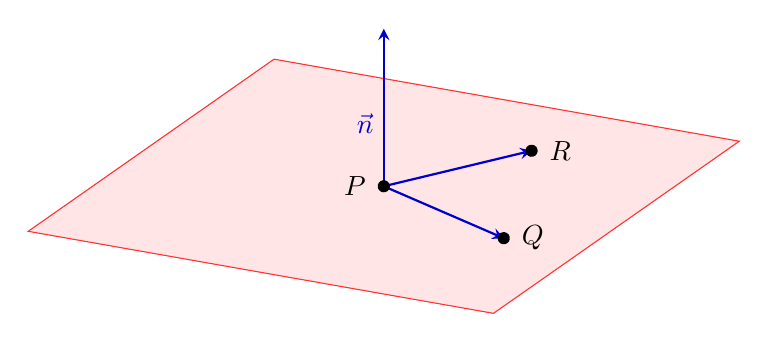
\begin{tikzpicture}[rotate=-10]
        \filldraw[draw=red!80,fill=red!10](-3,0,-3.5) -- (3,0,-3.5) -- (3,0,3.5) -- (-3,0,3.5) -- cycle;
        \draw[->,thick,blue!80!black](0,0,0) -- node[left, pos=0.4] {$\vect{n}$} (100:2);
        \draw[->,thick,blue!80!black](0,0,0) -- (2,0,1);
        \draw[->,thick,blue!80!black](0,0,0) -- (1,0,-2);
        \fill (0,0,0) circle [radius=2.2pt] node [left=3pt] {$P$};
        \fill (2,0,1) circle [radius=2.2pt] node [right=3pt] {$Q$};
        \fill (1,0,-2) circle [radius=2.2pt] node [right=3pt] {$R$};
      \end{tikzpicture}
    \end{center}
    Now we can easily obtain the normal equation from any point on the
    plane (say $P$) and the normal vector we just calculated:
    \begin{equation*}
      \startmat{r} 5 \\ -1 \\ 4 \stopmat
      \dotprod
      \startmat{r} x \\ y \\ z \stopmat
      =
      \startmat{r} 5 \\ -1 \\ 4 \stopmat
      \dotprod
      \startmat{r} 0 \\ 1 \\ 3 \stopmat
    \end{equation*}
    We get the standard equation by computing the dot products on the
    left- and right-hand sides:
    \begin{equation*}
      5x - y + 4z = 11.
    \end{equation*}
    It is worthwhile to double-check the answer by substituting each of
    the three original points $P$, $Q$, and $R$ into this equation.
    For example, for $Q=(2,-1,0)$, we obtain $5(2)-(-1)+4(0)$, which is
    indeed $11$.
  \end{solution}
 
\subsection*{Definition of the Cross Product}
 
\begin{definition}\label{def:crossproduct} Let $\vec{u=\begin{bmatrix}u_1\\u_2\\u_3\end{bmatrix}}$ and $\vec{v}=\begin{bmatrix}v_1\\v_2\\v_3\end{bmatrix}$ be vectors in $\RR^3$.  The \dfn{cross product} of $\vec{u}$ and $\vec{v}$, denoted by $\vec{u}\times\vec{v}$, is given by
\begin{align*}
\vec{u}\times\vec{v}&=(u_2v_3-u_3v_2)\vec{i}-(u_1v_3-u_3v_1)\vec{j}+(u_1v_2-u_2v_1)\vec{k} \\
&=(u_2v_3-u_3v_2)\begin{bmatrix}1\\0\\0\end{bmatrix}-(u_1v_3-u_3v_1)\begin{bmatrix}0\\1\\0\end{bmatrix}+(u_1v_2-u_2v_1)\begin{bmatrix}0\\0\\1\end{bmatrix}=\begin{bmatrix}u_2v_3-u_3v_2\\-u_1v_3+u_3v_1\\u_1v_2-u_2v_1\end{bmatrix}
\end{align*}
\end{definition}
 
This formula is much easier to remember when stated symbolically in terms of determinants.
$$\vec{u}\times \vec{v}=\begin{bmatrix}u_1\\u_2\\u_3\end{bmatrix}\times\begin{bmatrix}v_1\\v_2\\v_3\end{bmatrix}=\begin{vmatrix}\vec{i}&\vec{j}&\vec{k}\\u_1&u_2&u_3\\v_1&v_2&v_3\end{vmatrix}=\vec{i}\begin{vmatrix}u_2&u_3\\v_2&v_3\end{vmatrix}-\vec{j}\begin{vmatrix}u_1&u_3\\v_1&v_3\end{vmatrix}+\vec{k}\begin{vmatrix}u_1&u_2\\v_1&v_2\end{vmatrix} $$
 
\begin{example}\label{ex:crossproduct}
Find the cross product of $\vec{u}=\begin{bmatrix}3\\ -10\\ 2\end{bmatrix}$ and $\vec{v}=\begin{bmatrix}-2\\ 4\\ 7\end{bmatrix}$.
\begin{explanation}
\begin{align*}
\vec{u}\times \vec{v}&=
\begin{vmatrix}
\vec{i} & \vec{j} & \vec{k}\\
3 & -10 &2\\
-2 &4 &7
\end{vmatrix} =\vec{i}
\begin{vmatrix}
-10 & 2\\
4 & 7
\end{vmatrix} -\vec{j}
\begin{vmatrix}
3 & 2\\
-2 & 7
\end{vmatrix} +\vec{k}
\begin{vmatrix}
3 & -10\\
-2 & 4
\end{vmatrix}\\
&=\vec{i}\Big((-10)(7)-(2)(4)\Big)-\vec{j}\Big((3)(7)-(2)(-2)\Big)+\vec{k}\Big((3)(4)-(-10)(-2)\Big)\\
&=-78\vec{i}-25\vec{j}-8\vec{k}
=\begin{bmatrix}-78\\ -25\\ -8\end{bmatrix}
\end{align*}
\end{explanation}
\end{example}
 
\subsection*{Properties of the Cross Product}
 
% In the next example, we will use vectors $\vec{u}$ and $\vec{v}$ of Example \ref{ex:crossproduct}, and compute $\vec{v}\times\vec{u}$ to illustrate that the cross product is not commutative and to find a relationship between $\vec{u}\times\vec{v}$ and $\vec{v}\times \vec{u}$.  If you have already studied the effect that switching two rows of a matrix has on its determinant, you should be able to guess the outcome of the upcoming computation.
 
\begin{exploration}\label{init:crossproduct2}
What would happen if we took the cross product of the vectors in Example \ref{ex:crossproduct} but reversed the order?
 
Let $\vec{v}=\begin{bmatrix}-2\\ 4\\ 7\end{bmatrix}$ and $\vec{u}=\begin{bmatrix}3\\ -10\\ 2\end{bmatrix}$.
Recall that $\vec{u}\times\vec{v}=\begin{bmatrix}-78\\-25\\-8\end{bmatrix}$.  We need to compute $\vec{v}\times\vec{u}$.  If you have already studied the effect that switching two rows of a matrix has on its determinant, you should be able to guess the outcome of the upcoming computation.
\begin{align*}
\vec{v}\times \vec{u}&=
\begin{vmatrix}
\vec{i} & \vec{j} & \vec{k}\\
-2 &4 &7\\
3 & -10 &2
\end{vmatrix} =\vec{i}
\begin{vmatrix}
4 & 7\\
-10 & 2
\end{vmatrix} -\vec{j}
\begin{vmatrix}
-2 & 7\\
3 & 2
\end{vmatrix} +\vec{k}
\begin{vmatrix}
-2 & 4\\
3 & -10
\end{vmatrix}\\
&=\vec{i}\Big((4)(2)-(7)(-10)\Big)-\vec{j}\Big((-2)(2)-(7)(3)\Big)+\vec{k}\Big((-2)(-10)-(4)(3)\Big)\\
&=78\vec{i}+25\vec{j}+8\vec{k}
=\begin{bmatrix}78\\ 25\\ 8\end{bmatrix}=-(\vec{u}\times\vec{v})
\end{align*}
 
This computation shows that the cross product is an operation that is not commutative. It also suggests that switching the order of the vectors changes the sign of the result.
\end{exploration}
 
\begin{warning}The Cross Product is not a commutative operation.
\end{warning}
 
\begin{theorem}\label{th:corssuvnegcrossvu}
Let $\vec{u}$ and $\vec{v}$ be vectors in $\RR^3$, then
$$\vec{u}\times\vec{v}=-(\vec{v}\times\vec{u})$$
\end{theorem}

The next theorem lists two additional properties of the cross product.  Proofs of these properties are routine and are left to the reader.
\begin{theorem}\label{th:crossproductproperties}
Let $\vec{u}$, $\vec{v}$ and $\vec{w}$ be vectors in $\mathbb{R}^3$, and $k$ be a scalar, then\\
\begin{enumerate}
\item\label{item:scalarassocofcrossprod} Scalar Associativity
$$(k\vec{u})\times \vec{v}=\vec{u}\times (k\vec{v})=k(\vec{u}\times \vec{v})$$
\item\label{item:distofrossprod} Distributivity
$$(\vec{u}+\vec{v})\times \vec{w}=\vec{u}\times \vec{w}+\vec{v}\times \vec{w}$$
$$\vec{u}\times (\vec{v}+\vec{w})=\vec{u}\times \vec{v}+\vec{u}\times \vec{w}$$
\end{enumerate}
\end{theorem}
 
The cross product has several important geometric properties. The following problems give us a glimpse of these properties.
 
\begin{exploration}\label{init:ijkcrossproducts}
Compute the following products:
$$\vec{i}\times\vec{j}=\begin{bmatrix}\answer{0}\\\answer{0}\\\answer{1}\end{bmatrix},\quad\vec{j}\times\vec{k}=\begin{bmatrix}\answer{1}\\\answer{0}\\\answer{0}\end{bmatrix}$$
 
For the two vectors in each product, sketch the vectors together with the product vector.  What do you observe about the relationship between the cross product and the plane determined by the two vectors in the product? 
\begin{hint}
$\vec{i}\times\vec{j}=\vec{k}$.  Vector $\vec{k}$ is orthogonal to both $\vec{i}$ and $\vec{j}$. 
\end{hint}
 
 
 
\end{exploration}
 
\subsubsection*{Orthogonality Property}
\begin{exploration}\label{init:orthofcorssproduct}
In this problem we will return to vectors of $\vec{v}=\begin{bmatrix}-2\\ 4\\ 7\end{bmatrix}$ and $\vec{u}=\begin{bmatrix}3\\ -10\\ 2\end{bmatrix}$ of Example \ref{ex:crossproduct} and Exploration Problem \ref{init:crossproduct2}.  We know that
$$\vec{u}\times\vec{v}=\begin{bmatrix}-78\\-25\\-8\end{bmatrix}\quad\text{and}\quad\vec{v}\times\vec{u}=\begin{bmatrix}78\\25\\8\end{bmatrix}$$
We will now compute the dot product of $\vec{v}\times\vec{u}$ with each of the original vectors $\vec{u}$ and $\vec{v}$.
$$\vec{u}\dotp(\vec{v}\times\vec{u})=\begin{bmatrix}3\\ -10\\ 2\end{bmatrix}\dotp\begin{bmatrix}78\\25\\8\end{bmatrix}=0$$
$$\vec{v}\dotp(\vec{v}\times\vec{u})=\begin{bmatrix}-2\\ 4\\ 7\end{bmatrix}\dotp\begin{bmatrix}78\\25\\8\end{bmatrix}=0$$
It is also easy to verify that $\vec{u}\dotp(\vec{u}\times\vec{v})=0$ and $\vec{v}\dotp(\vec{u}\times\vec{v})=0$.  Recall that the dot product of two vectors is $0$ if and only if the two vectors are orthogonal.
We conclude that, at least in this case, the cross product of two vectors is orthogonal to each of the vectors. 
 
\end{exploration}
 
It turns out that the orthogonality property illustrated by Exploration Problems \ref{init:ijkcrossproducts} and \ref{init:orthofcorssproduct}  holds in general.  We state it as a theorem.
 
\begin{theorem}\label{th:crossproductorthtouandv}
Let $\vec{u}$ and $\vec{v}$ be vectors of $\RR^3$, then $\vec{u}\times\vec{v}$ is orthogonal to both $\vec{u}$ and $\vec{v}$.
\end{theorem}

 
\subsubsection*{Cross Product and the Angle between Vectors}
Recall that the dot product of $\vec{u}$ and $\vec{v}$ is related to the angle $\theta$ between $\vec{u}$ and $\vec{v}$ by the following formula
\begin{align}\label{eq:dotproductformula}\vec{u}\dotp\vec{v}=\norm{\vec{u}}\norm{\vec{v}}\cos\theta\end{align}
We will derive an analogous result for the cross product.  To do so, we will need the following Lemma.
 
\begin{lemma}\label{lemma:crossprodmagnitude}
Let $\vec{u}$ and $\vec{v}$ be vectors in $\RR^3$.  Then
$$\norm{\vec{u}\times\vec{v}}^2=\norm{\vec{u}}^2\norm{\vec{v}}^2-(\vec{u}\dotp\vec{v})^2$$
\end{lemma}

 
The following theorem establishes a relationship between the magnitude of the cross product, the magnitudes of the two vectors involved in the cross product and the angle between the two vectors.  It is important to note that  the identity in this theorem involves the magnitude of the cross product, not the cross product itself.
 
\begin{theorem}\label{th:crossproductsin}
Let $\vec{u}$ and $\vec{v}$ be vectors in $\RR^3$. Let $\theta$ be the angle between $\vec{u}$ and $\vec{v}$ such that $0\leq\theta\leq \pi$. Then
$$\norm{\vec{u}\times\vec{v}}=\norm{\vec{u}}\norm{\vec{v}}\sin\theta$$
\end{theorem}
\begin{proof}
We have
\begin{align*}
\norm{\vec{u}\times\vec{v}}^2&=\norm{\vec{u}}^2\norm{\vec{v}}^2-(\vec{u}\dotp\vec{v})^2\\
&=\norm{\vec{u}}^2\norm{\vec{v}}^2-(\norm{\vec{u}}\norm{\vec{v}}\cos \theta)^2\\
&=\norm{\vec{u}}^2\norm{\vec{v}}^2-\norm{\vec{u}}^2\norm{\vec{v}}^2\cos^2\theta\\
&=\norm{\vec{u}}^2\norm{\vec{v}}^2(1-\cos^2\theta)\\
&=\norm{\vec{u}}^2\norm{\vec{v}}^2\sin^2\theta
\end{align*}
Observe that all magnitudes are non-negative.  Also, $\sin\theta\geq 0$ because $0\leq\theta\leq \pi$.  Taking the square root of both sides give us
$$\norm{\vec{u}\times\vec{v}}=\norm{\vec{u}}\norm{\vec{v}}\sin\theta$$
\end{proof}
 

\end{document}